\documentclass[tikz]{standalone}
\usetikzlibrary{decorations.markings,arrows.meta}
\begin{document}
      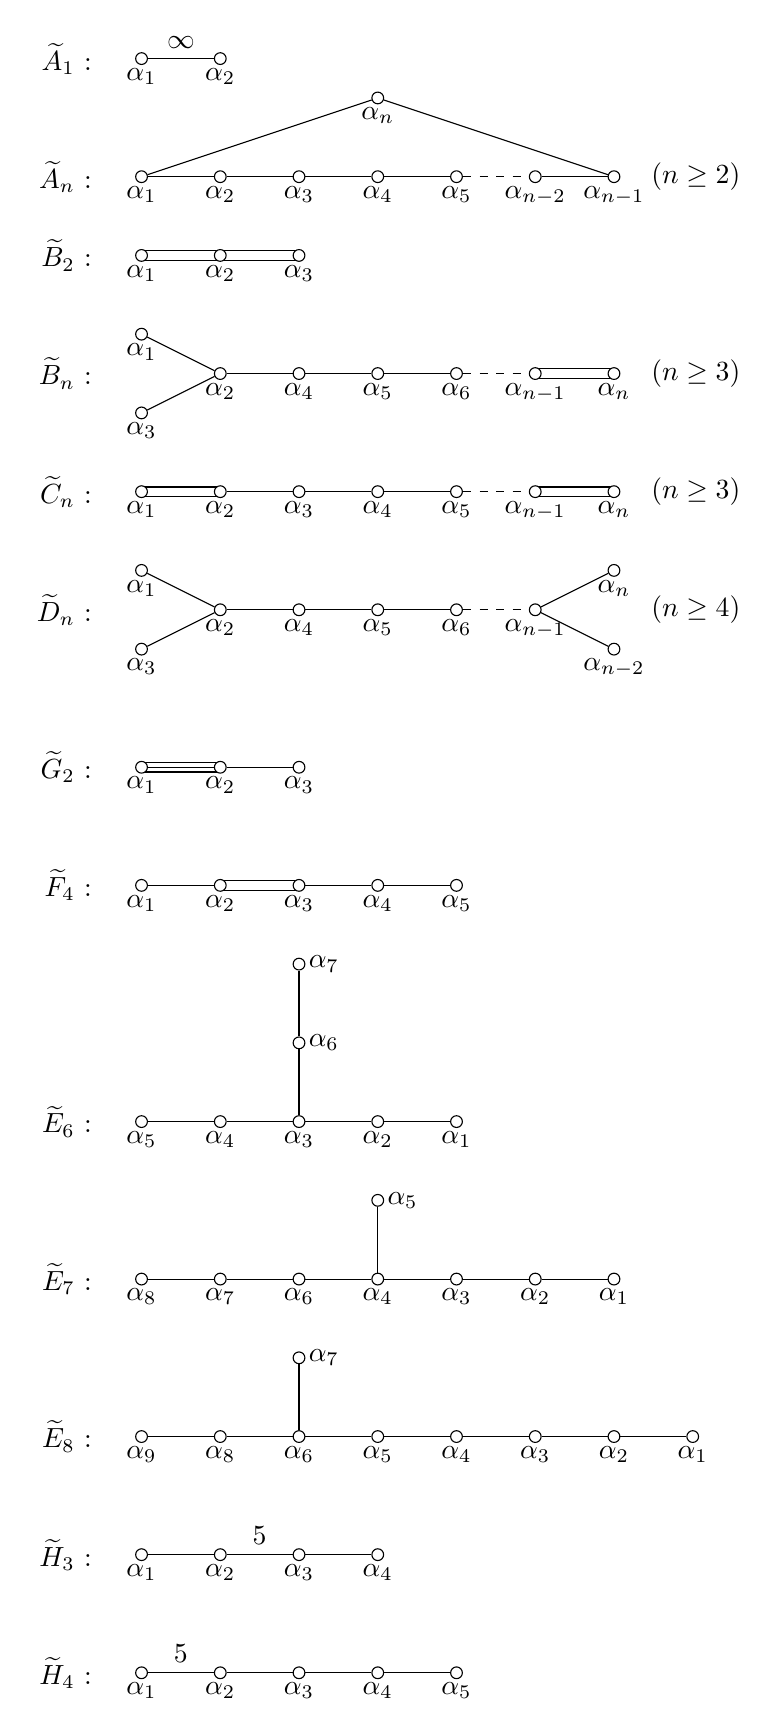
\begin{tikzpicture}
        % A_1
        \foreach \i in {1,2}
					\node[circle, draw, fill=white, inner sep=1.5pt] (\i) at (\i,1.5) {};
				\draw (1) -- node[midway, above]{$\infty$} (2);
        \node[below] at (1) {$\alpha_1$};
        \node[below] at (2) {$\alpha_2$};
        \node[left] at (1) {$\widetilde{A}_1$ : \mbox{\hspace{10pt}}};

        % A_n
        \foreach \i in {1,...,7}
					\node[circle, draw, fill=white, inner sep=1.5pt] (\i) at (\i,0) {};
        \node[circle, draw, fill=white, inner sep=1.5pt] (8) at (4,1) {};
				\foreach \i in {1,...,4,6}
					\draw (\i) -- (\the\numexpr\i+1\relax);
				\draw[dashed] (5) -- (6);
        \node[below] at (1) {$\alpha_1$};
        \node[below] at (2) {$\alpha_2$};
        \node[below] at (3) {$\alpha_3$};
        \node[below] at (4) {$\alpha_4$};
        \node[below] at (5) {$\alpha_5$};
        \node[below] at (6) {$\alpha_{n-2}$};
        \node[below] at (7) {$\alpha_{n-1}$};
        \node[below] at (8) {$\alpha_n$};
        \draw (1) -- (8);
        \draw (7) -- (8);
        \node[left] at (1) {$\widetilde{A}_n$ : \mbox{\hspace{10pt}}};
        \node[right] at (7) {\mbox{\hspace{10pt}}$(n \ge 2)$};

        % B_2
        \draw[double distance=3pt, postaction={decorate}] (1, -1) -- (2, -1);
        \draw[double distance=3pt, postaction={decorate}] (2, -1) -- (3, -1);
        \foreach \i in {1,...,3}
					\node[circle, draw, fill=white, inner sep=1.5pt] (\i) at (\i,-1) {};
        \node[below] at (1) {$\alpha_1$};
        \node[below] at (2) {$\alpha_2$};
        \node[below] at (3) {$\alpha_3$};
        \node[left] at (1) {$\widetilde{B}_2$ : \mbox{\hspace{10pt}}};

        % B_n
        \draw[double distance=3pt, postaction={decorate}] (6, -2.5) -- (7, -2.5);
        \foreach \i in {2,...,7}
					\node[circle, draw, fill=white, inner sep=1.5pt] (\i) at (\i,-2.5) {};
				\foreach \i in {2,...,4}
					\draw (\i) -- (\the\numexpr\i+1\relax);
				\draw[dashed] (5) -- (6);
				\node[circle, draw, fill=white, inner sep=1.5pt] (0) at (1,-2) {};
				\node[circle, draw, fill=white, inner sep=1.5pt] (1) at (1,-3) {};
				\foreach \i in {0,1}
					\draw (\i) -- (2);
        \node[below] at (0) {$\alpha_1$};
        \node[below] at (1) {$\alpha_3$};
        \node[below] at (2) {$\alpha_2$};
        \node[below] at (3) {$\alpha_4$};
        \node[below] at (4) {$\alpha_5$};
        \node[below] at (5) {$\alpha_6$};
        \node[below] at (6) {$\alpha_{n-1}$};
        \node[below] at (7) {$\alpha_n$};
        \node[left] at (1, -2.5) {$\widetilde{B}_n$ : \mbox{\hspace{10pt}}};
        \node[right] at (7) {\mbox{\hspace{10pt}}$(n \ge 3)$};

        % C_n
				\draw[double distance=3pt, postaction={decorate}] (1, -4) -- (2, -4);
        \draw[double distance=3pt, postaction={decorate}] (6, -4) -- (7, -4);
				\foreach \i in {1,...,7}
					\node[circle, draw, fill=white, inner sep=1.5pt] (\i) at (\i,-4) {};
				\foreach \i in {2,...,4}
					\draw (\i) -- (\the\numexpr\i+1\relax);
				\draw[dashed] (5) -- (6);
        \node[below] at (1) {$\alpha_1$};
        \node[below] at (2) {$\alpha_2$};
        \node[below] at (3) {$\alpha_3$};
        \node[below] at (4) {$\alpha_4$};
        \node[below] at (5) {$\alpha_5$};
        \node[below] at (6) {$\alpha_{n-1}$};
        \node[below] at (7) {$\alpha_n$};
        \node[left] at (1) {$\widetilde{C}_n$ : \mbox{\hspace{10pt}}};
        \node[right] at (7) {\mbox{\hspace{10pt}}$(n \ge 3)$};

        % D_n
        \foreach \i in {2,...,6}
					\node[circle, draw, fill=white, inner sep=1.5pt] (\i) at (\i,-5.5) {};
				\foreach \i in {2,...,4}
					\draw (\i) -- (\the\numexpr\i+1\relax);
				\draw[dashed] (5) -- (6);
				\node[circle, draw, fill=white, inner sep=1.5pt] (0) at (1,-5) {};
				\node[circle, draw, fill=white, inner sep=1.5pt] (1) at (1,-6) {};
        \node[circle, draw, fill=white, inner sep=1.5pt] (7) at (7,-5) {};
				\node[circle, draw, fill=white, inner sep=1.5pt] (8) at (7,-6) {};
				\foreach \i in {0,1}
					\draw (\i) -- (2);
        \foreach \i in {7,8}
					\draw (\i) -- (6);
        \node[below] at (0) {$\alpha_1$};
        \node[below] at (1) {$\alpha_3$};
        \node[below] at (2) {$\alpha_2$};
        \node[below] at (3) {$\alpha_4$};
        \node[below] at (4) {$\alpha_5$};
        \node[below] at (5) {$\alpha_6$};
        \node[below] at (6) {$\alpha_{n-1}$};
        \node[below] at (7) {$\alpha_n$};
        \node[below] at (8) {$\alpha_{n-2}$};
        \node[left] at (1, -5.5) {$\widetilde{D}_n$ : \mbox{\hspace{10pt}}};
        \node[right] at (7, -5.5) {\mbox{\hspace{10pt}}$(n \ge 4)$};

        % G_2
        \draw[double distance=3pt, postaction={decorate}] (1, -7.5) -- (2, -7.5);
        \foreach \i in {1,2,3}
					\node[circle, draw, fill=white, inner sep=1.5pt] (\i) at (\i,-7.5) {};
				\draw (1) -- (2);
        \draw (2) -- (3);
        \node[below] at (1) {$\alpha_1$};
        \node[below] at (2) {$\alpha_2$};
        \node[below] at (3) {$\alpha_3$};
        \node[left] at (1) {$\widetilde{G}_2$ : \mbox{\hspace{10pt}}};

        % F_4
				\draw[double distance=3pt, postaction={decorate}] (2, -9) -- (3, -9);
        \foreach \i in {1,...,5}
					\node[circle, draw, fill=white, inner sep=1.5pt] (\i) at (\i,-9) {};
				\foreach \i in {1,3,4}
					\draw (\i) -- (\the\numexpr\i+1\relax);
        \node[below] at (1) {$\alpha_1$};
        \node[below] at (2) {$\alpha_2$};
        \node[below] at (3) {$\alpha_3$};
        \node[below] at (4) {$\alpha_4$};
        \node[below] at (5) {$\alpha_5$};
        \node[left] at (1) {$\widetilde{F}_4$ : \mbox{\hspace{10pt}}};

        % E_6
        \foreach \i in {1,...,5}
					\node[circle, draw, fill=white, inner sep=1.5pt] (\i) at (\i,-12) {};
				\node[circle, draw, fill=white, inner sep=1.5pt] (8) at (3,-11) {};
        \node[circle, draw, fill=white, inner sep=1.5pt] (9) at (3,-10) {};
				\foreach \i in {1,...,4}
					\draw (\i) -- (\the\numexpr\i+1\relax);
				\draw (3) -- (8);
        \draw (8) -- (9);
        \node[below] at (1) {$\alpha_5$};
        \node[right] at (8) {$\alpha_6$};
        \node[below] at (2) {$\alpha_4$};
        \node[below] at (3) {$\alpha_3$};
        \node[below] at (4) {$\alpha_2$};
        \node[below] at (5) {$\alpha_1$};
        \node[right] at (9) {$\alpha_7$};
        \node[left] at (1) {$\widetilde{E}_6$ : \mbox{\hspace{10pt}}};

        % E_7
        \foreach \i in {1,...,7}
					\node[circle, draw, fill=white, inner sep=1.5pt] (\i) at (\i,-14) {};
				\node[circle, draw, fill=white, inner sep=1.5pt] (8) at (4,-13) {};
				\foreach \i in {1,...,6}
					\draw (\i) -- (\the\numexpr\i+1\relax);
				\draw (4) -- (8);
        \node[below] at (1) {$\alpha_8$};
        \node[right] at (8) {$\alpha_5$};
        \node[below] at (2) {$\alpha_7$};
        \node[below] at (3) {$\alpha_6$};
        \node[below] at (4) {$\alpha_4$};
        \node[below] at (5) {$\alpha_3$};
        \node[below] at (6) {$\alpha_2$};
        \node[below] at (7) {$\alpha_1$};
        \node[left] at (1) {$\widetilde{E}_7$ : \mbox{\hspace{10pt}}};

        % E_8
        \foreach \i in {1,...,8}
					\node[circle, draw, fill=white, inner sep=1.5pt] (\i) at (\i,-16) {};
				\node[circle, draw, fill=white, inner sep=1.5pt] (9) at (3,-15) {};
				\foreach \i in {1,...,7}
					\draw (\i) -- (\the\numexpr\i+1\relax);
				\draw (3) -- (9);
        \node[below] at (1) {$\alpha_9$};
        \node[right] at (9) {$\alpha_7$};
        \node[below] at (2) {$\alpha_8$};
        \node[below] at (3) {$\alpha_6$};
        \node[below] at (4) {$\alpha_5$};
        \node[below] at (5) {$\alpha_4$};
        \node[below] at (6) {$\alpha_3$};
        \node[below] at (7) {$\alpha_2$};
        \node[below] at (8) {$\alpha_1$};
        \node[left] at (1) {$\widetilde{E}_8$ : \mbox{\hspace{10pt}}};

        % H_3
        \foreach \i in {1,...,4}
					\node[circle, draw, fill=white, inner sep=1.5pt] (\i) at (\i,-17.5) {};
        \draw (1) -- (2);
				\draw (2) -- node[midway, above]{$5$} (3);
        \draw (3) -- (4);
        \node[below] at (1) {$\alpha_1$};
        \node[below] at (2) {$\alpha_2$};
        \node[below] at (3) {$\alpha_3$};
        \node[below] at (4) {$\alpha_4$};
        \node[left] at (1) {$\widetilde{H}_3$ : \mbox{\hspace{10pt}}};

        % H_4
        \foreach \i in {1,...,5}
					\node[circle, draw, fill=white, inner sep=1.5pt] (\i) at (\i,-19) {};
				\draw (1) -- node[midway, above]{$5$} (2);
        \draw (2) -- (3);
        \draw (3) -- (4);
        \draw (4) -- (5);
        \node[below] at (1) {$\alpha_1$};
        \node[below] at (2) {$\alpha_2$};
        \node[below] at (3) {$\alpha_3$};
        \node[below] at (4) {$\alpha_4$};
        \node[below] at (5) {$\alpha_5$};
        \node[left] at (1) {$\widetilde{H}_4$ : \mbox{\hspace{10pt}}};
      \end{tikzpicture}
\end{document}
